\appendix{Other results}\label{app:results}
All remaining image results are in this section. 


%%%%%%%%%%%%%%%%%%%%%%%%%%%%%%%%%%%%%%%%%%%%%%%%%
%SQE Results per forecaster
%%%%%%%%%%%%%%%%%%%%%%%%%%%%%%%%%%%%%%%%%%%%%%%%%
\bigskip
\noindent \textbf{SQEONAN Results per forecaster} \\
%merl
\begin{figure}[!h]
	\begin{center}
		\subfigure[] {
			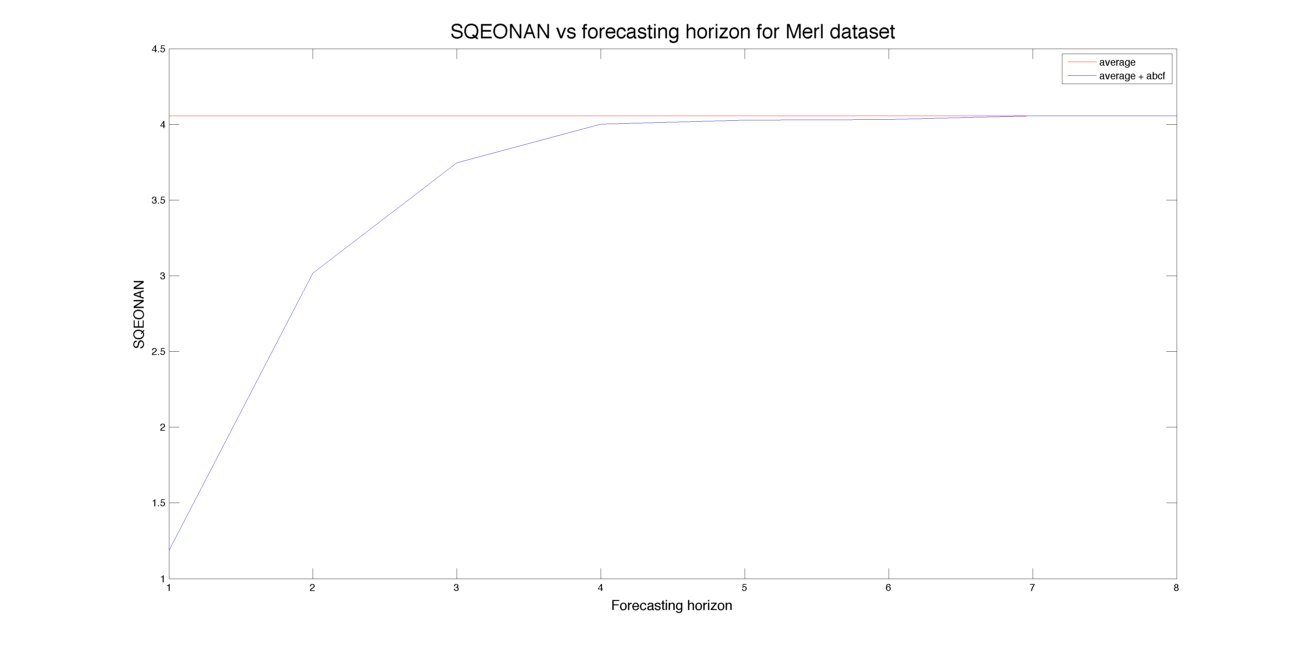
\includegraphics[width=0.37\textwidth]{sqe_merl_avg.png}
		}
		\subfigure[] {
			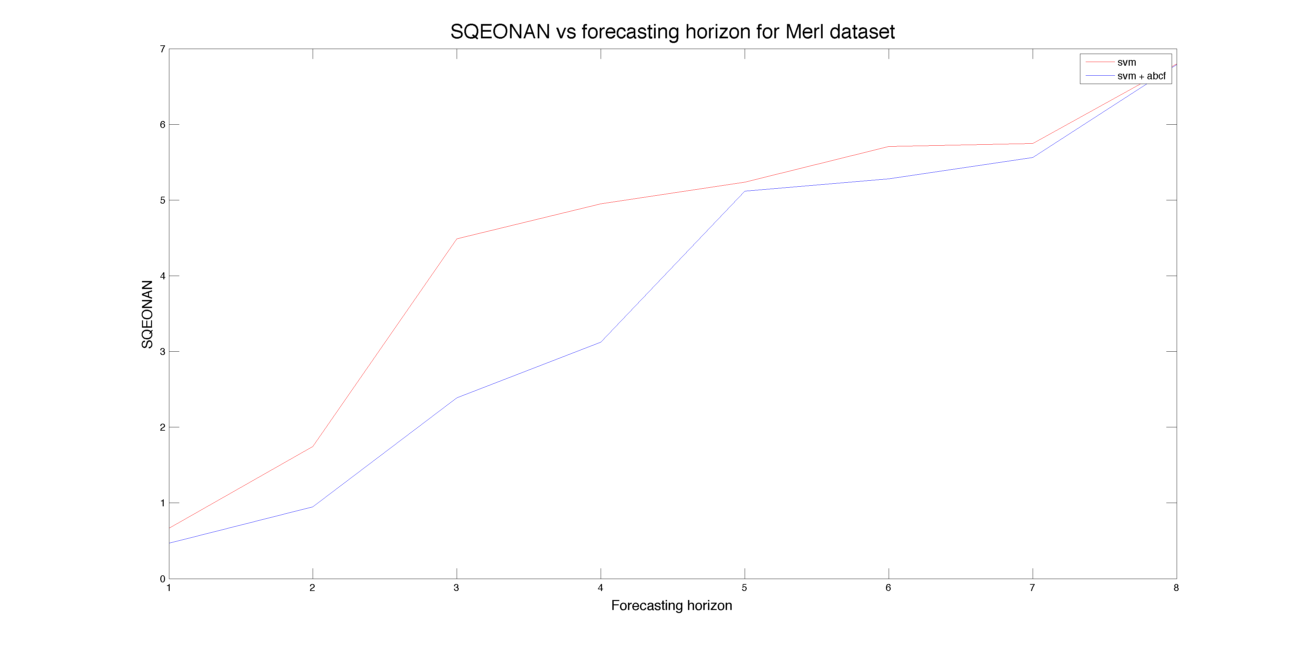
\includegraphics[width=0.37\textwidth]{sqe_merl_svm.png}
		} \\
		\subfigure[] {
			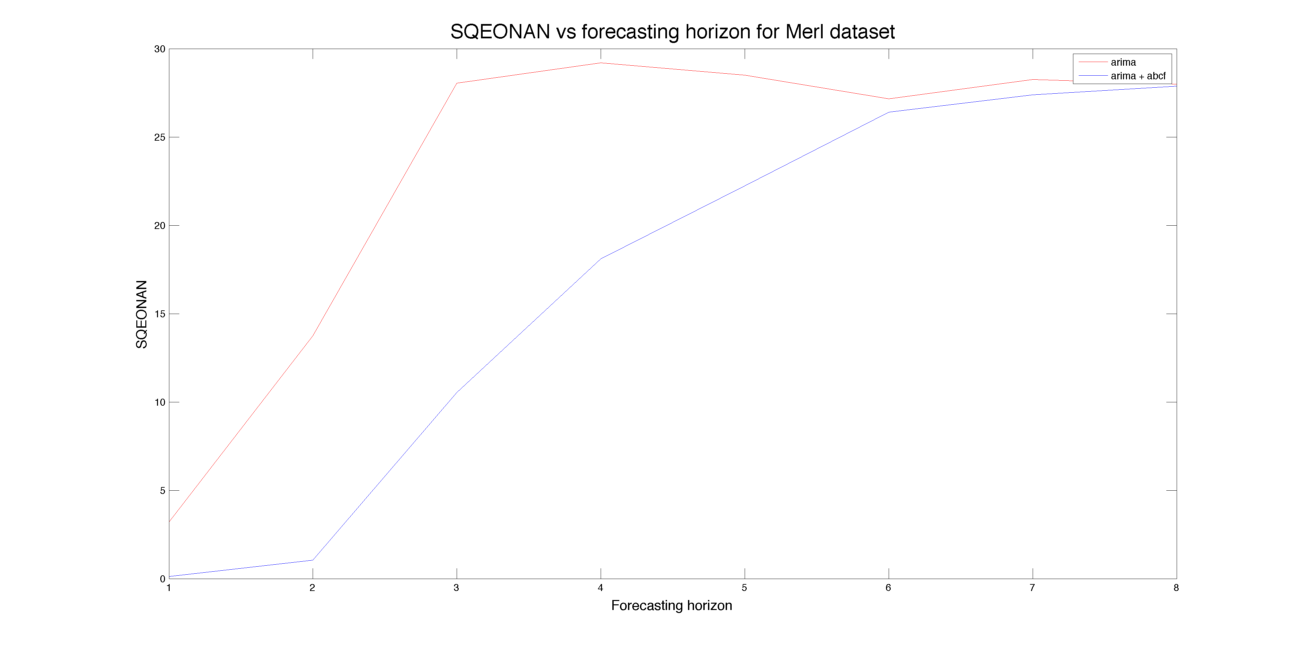
\includegraphics[width=0.37\textwidth]{sqe_merl_arima.png}
		}
		\subfigure[] {
			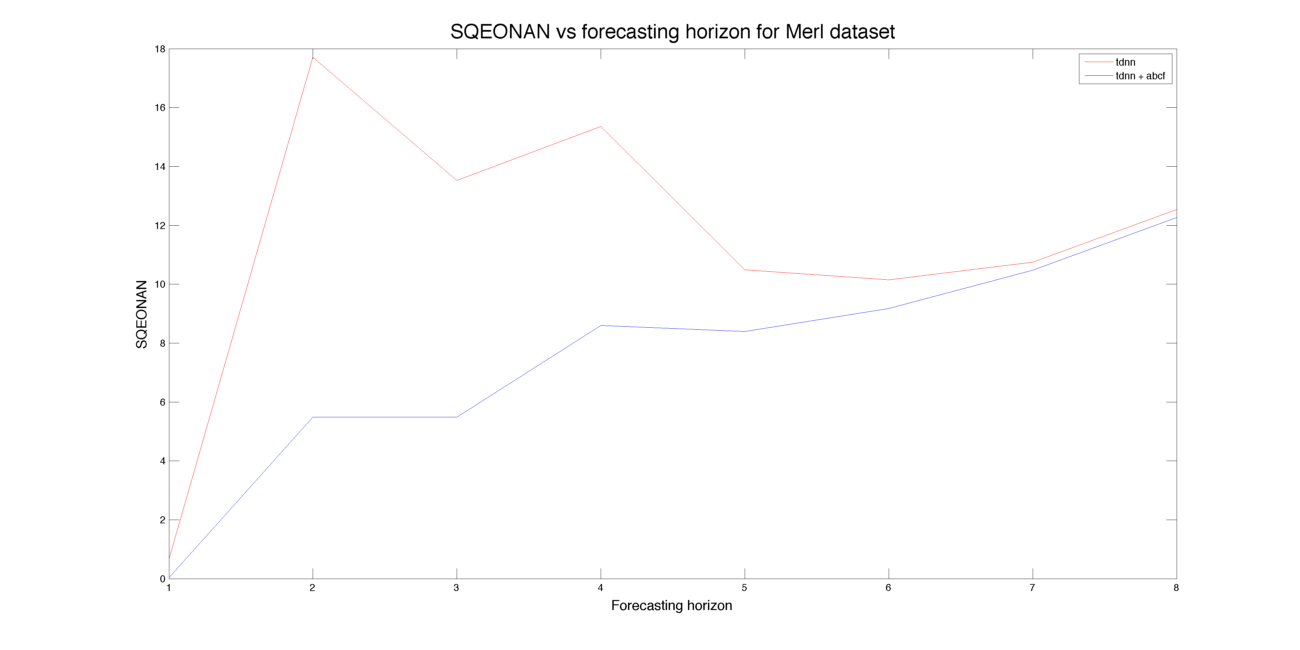
\includegraphics[width=0.37\textwidth]{sqe_merl_tdnn.png}
		}
	\end{center}
	\caption{Results for the four base forecasting algorithms for the Brown Hall dataset and the improvements to SQEONAN from using our ABCF algorithm}
	\label{fig:sqe_merl_results}
\end{figure}

%brown
\begin{figure}[!h]
	\begin{center}
		\subfigure[] {
			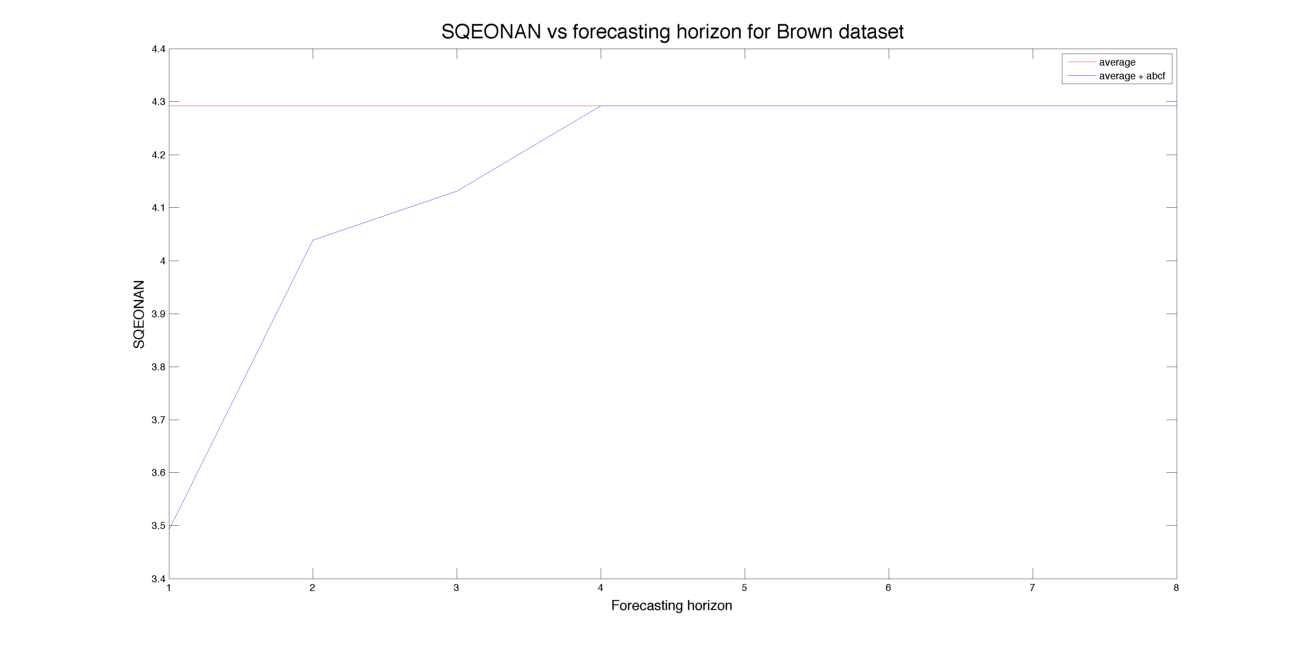
\includegraphics[width=0.37\textwidth]{sqe_brown_avg.png}
		}
		\subfigure[] {
			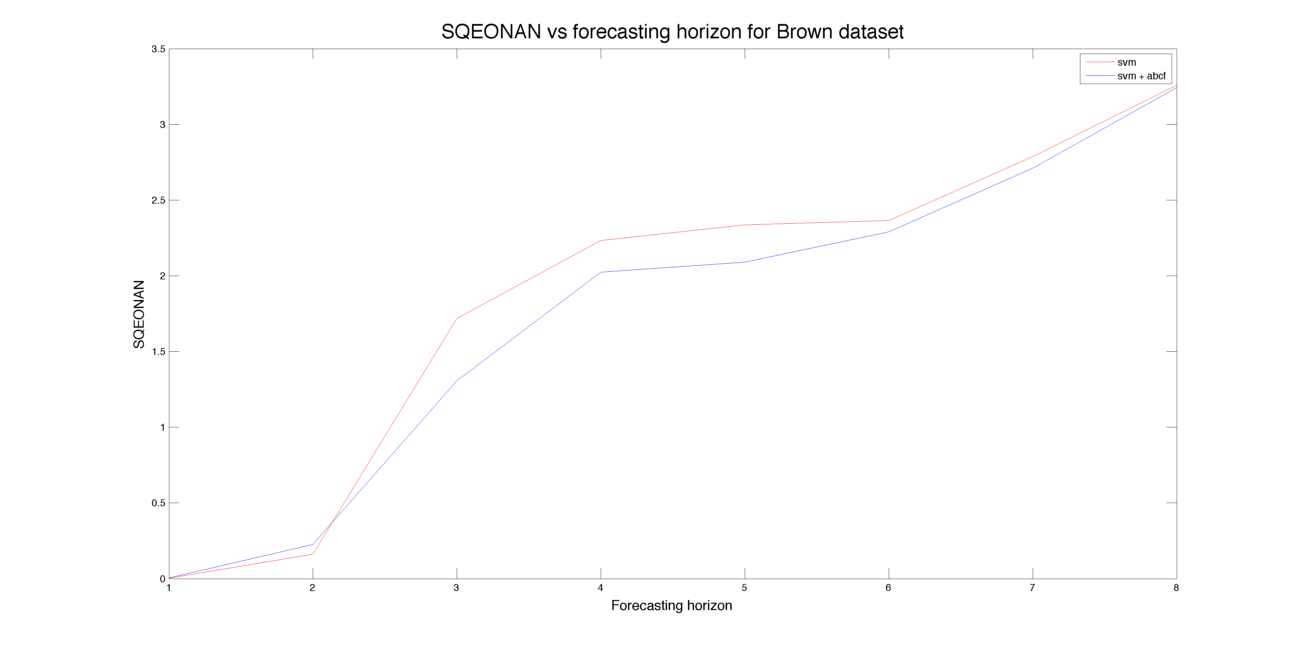
\includegraphics[width=0.37\textwidth]{sqe_brown_svm.png}
		} \\
		\subfigure[] {
			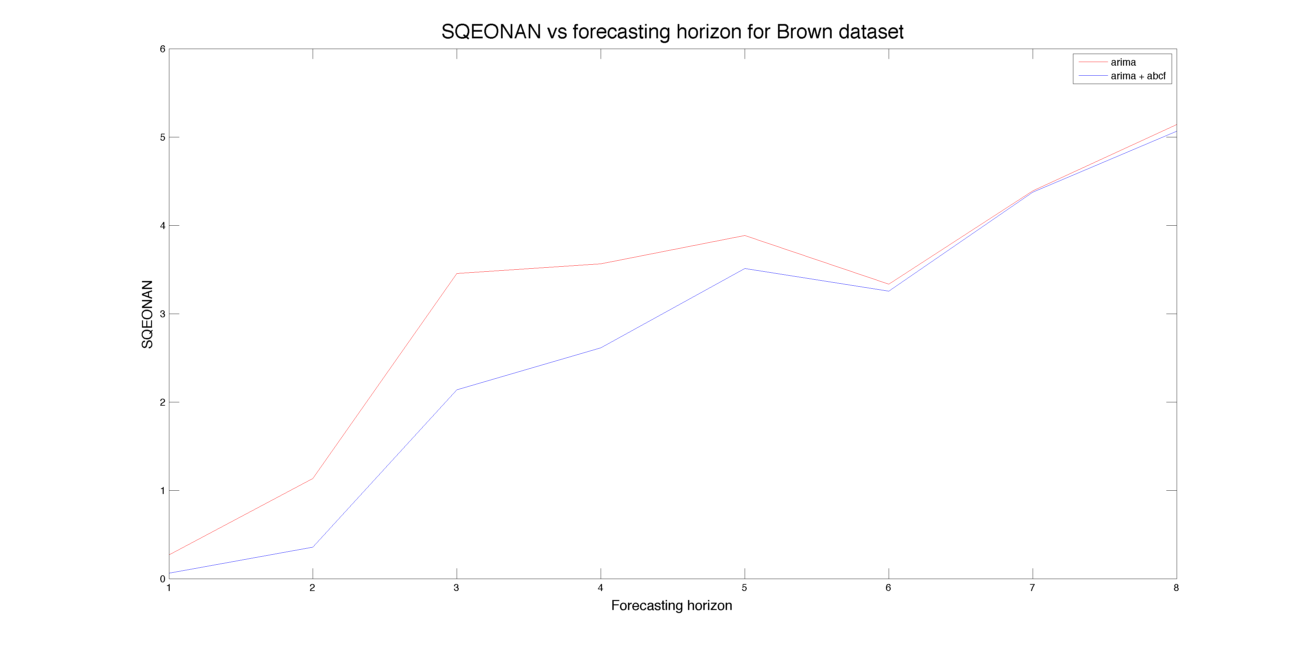
\includegraphics[width=0.37\textwidth]{sqe_brown_arima.png}
		}
		\subfigure[] {
			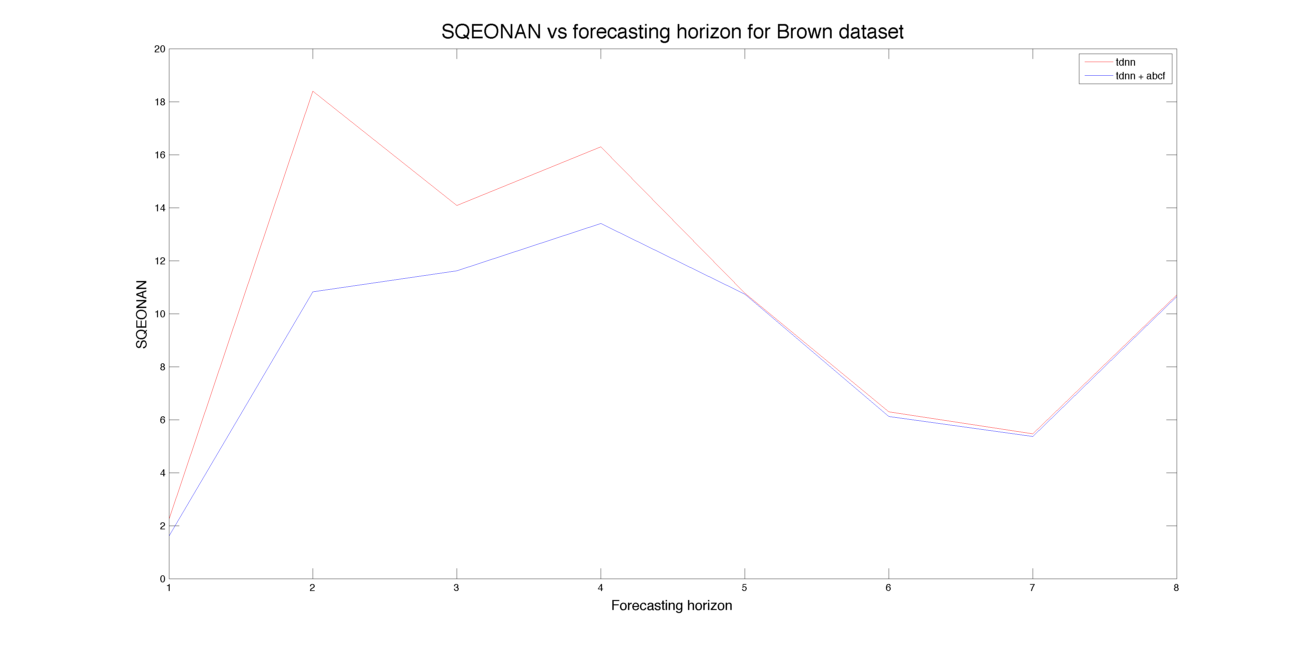
\includegraphics[width=0.37\textwidth]{sqe_brown_tdnn.png}
		}
	\end{center}
	\caption{Results for the four base forecasting algorithms for the Brown Hall dataset and the improvements to SQEONAN from using our ABCF algorithm}
	\label{fig:sqe_brown_results}
\end{figure}

%denver
\begin{figure}[!h]
	\begin{center}
		\subfigure[] {
			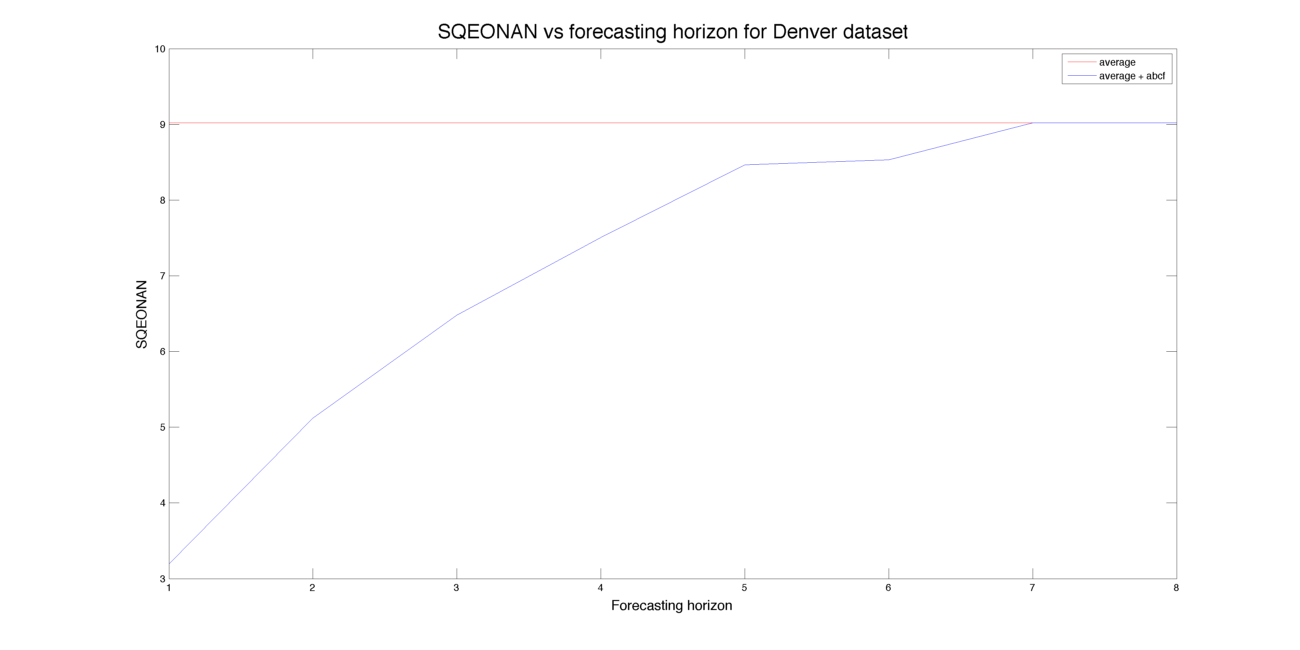
\includegraphics[width=0.37\textwidth]{sqe_denver_avg.png}
		}
		\subfigure[] {
			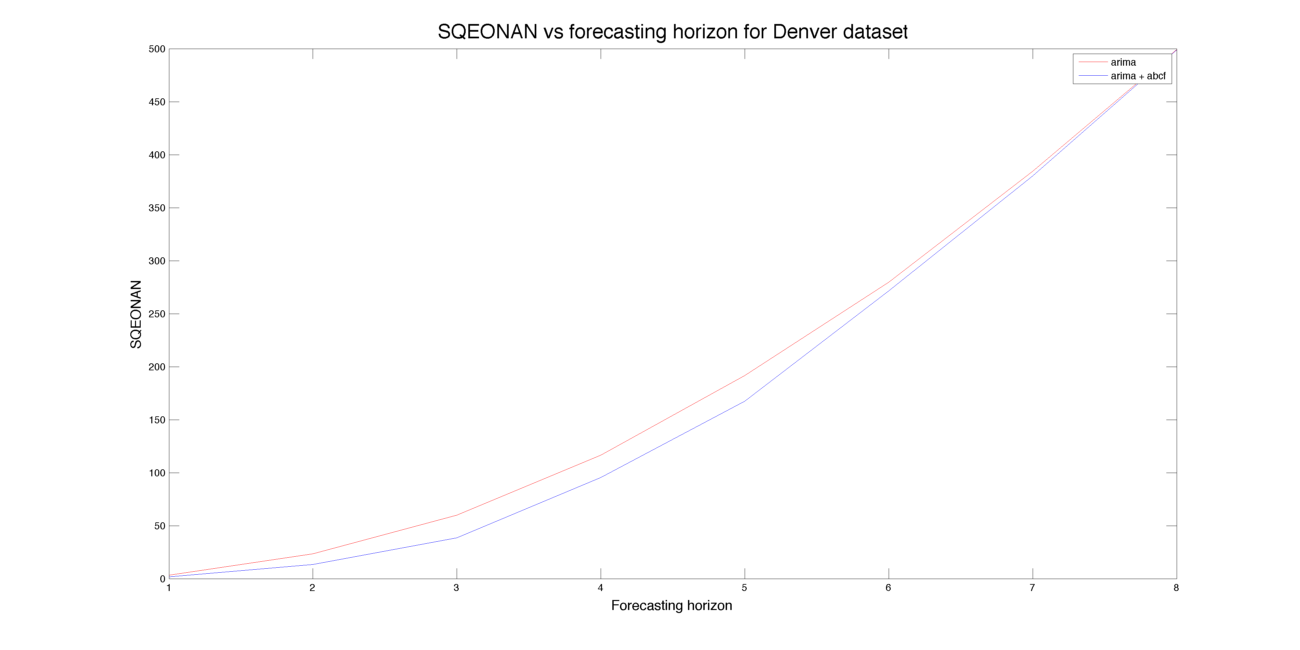
\includegraphics[width=0.37\textwidth]{sqe_denver_svm.png}
		} \\
		\subfigure[] {
			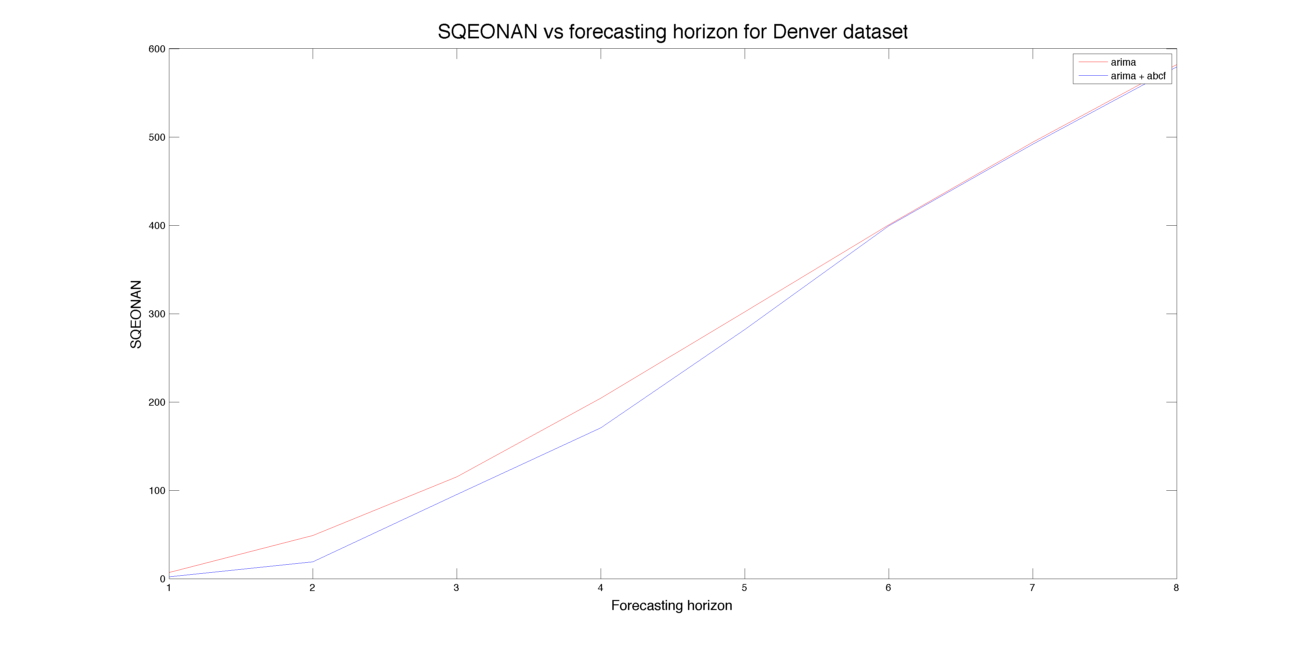
\includegraphics[width=0.37\textwidth]{sqe_denver_arima.png}
		}
		\subfigure[] {
			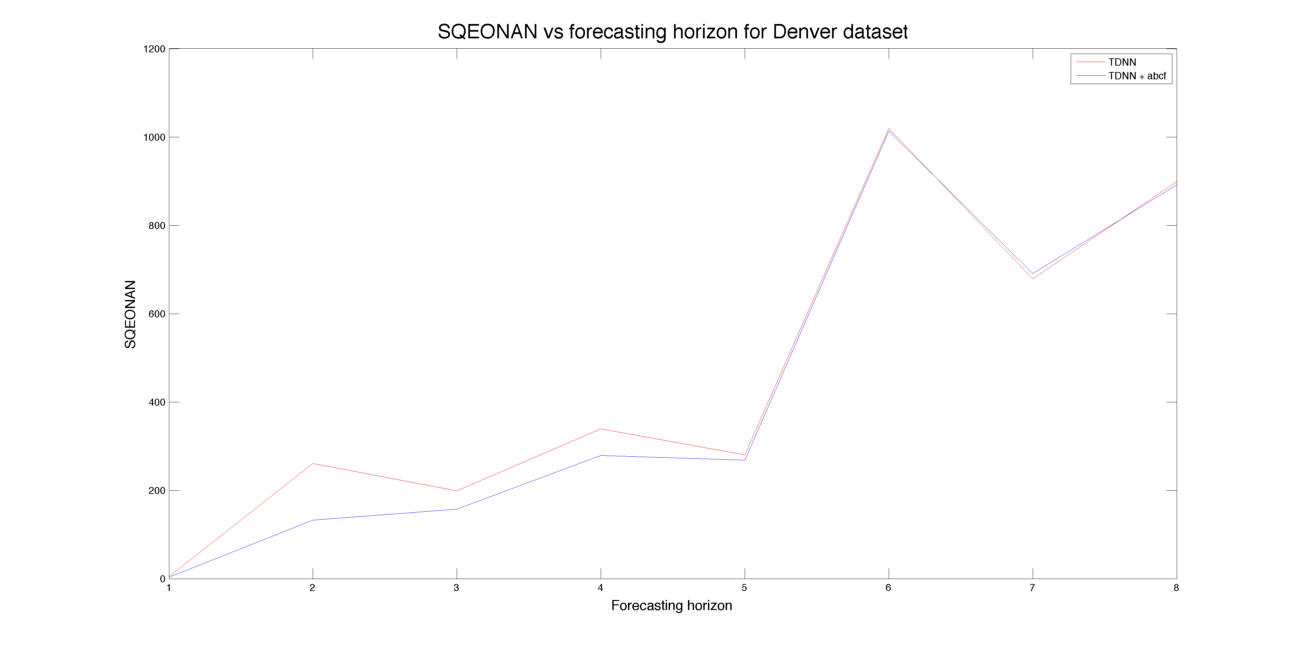
\includegraphics[width=0.37\textwidth]{sqe_denver_tdnn.png}
		}
	\end{center}
	\caption{Results for the four base forecasting algorithms for the Denver dataset and the improvements to SQEONAN from using our ABCF algorithm}
	\label{fig:sqe_denver_results}
\end{figure}

\newpage

%%%%%%%%%%%%%%%%%%%%%%%%%%%%%%%%%%%%%%%%%%%%%%%%%
%RMSE Results per forecaster
%%%%%%%%%%%%%%%%%%%%%%%%%%%%%%%%%%%%%%%%%%%%%%%%%
\bigskip 
\noindent \textbf{RMSE Results per forecaster} \\

%merl
\begin{figure}[!h]
	\begin{center}
		\subfigure[] {
			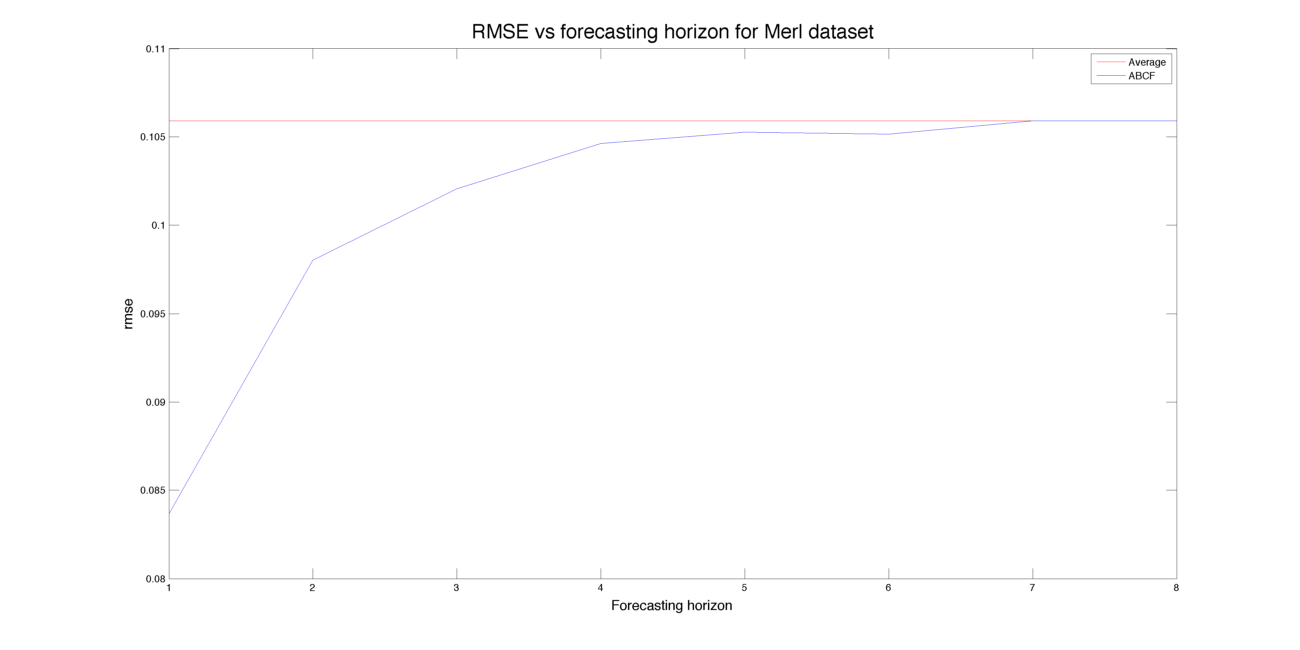
\includegraphics[width=0.37\textwidth]{rmse_merl_avg.png}
		}
		\subfigure[] {
			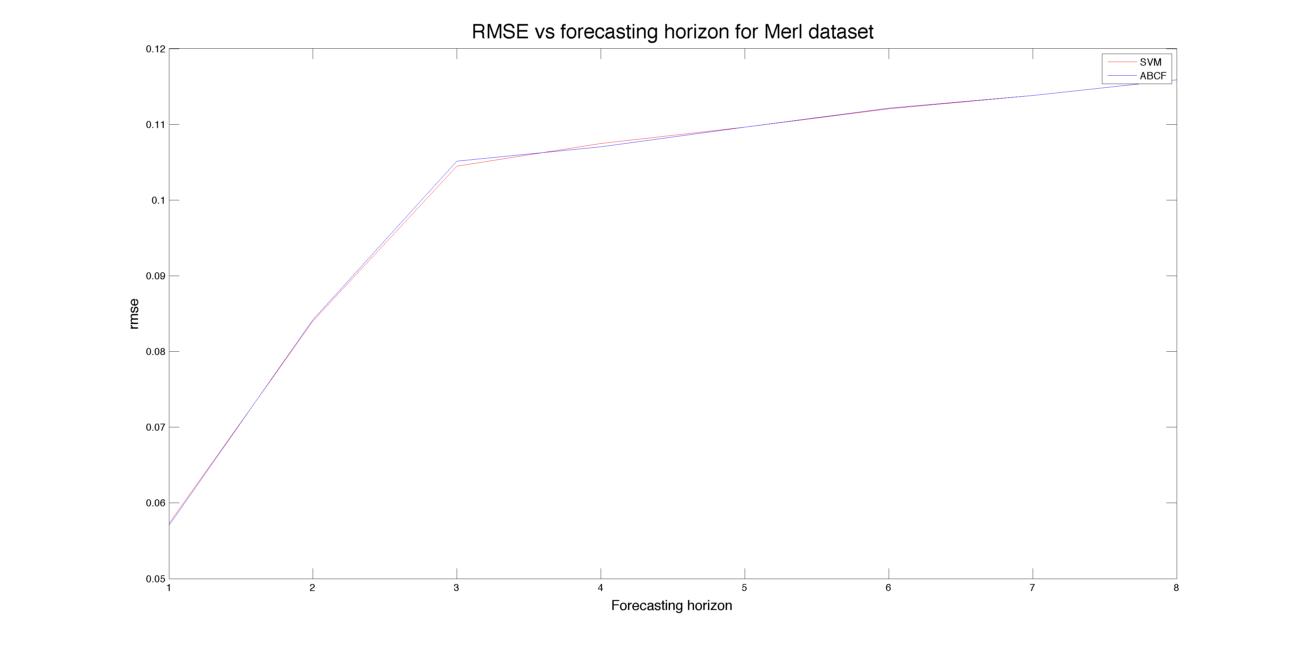
\includegraphics[width=0.37\textwidth]{rmse_merl_svm.png}
		} \\
		\subfigure[] {
			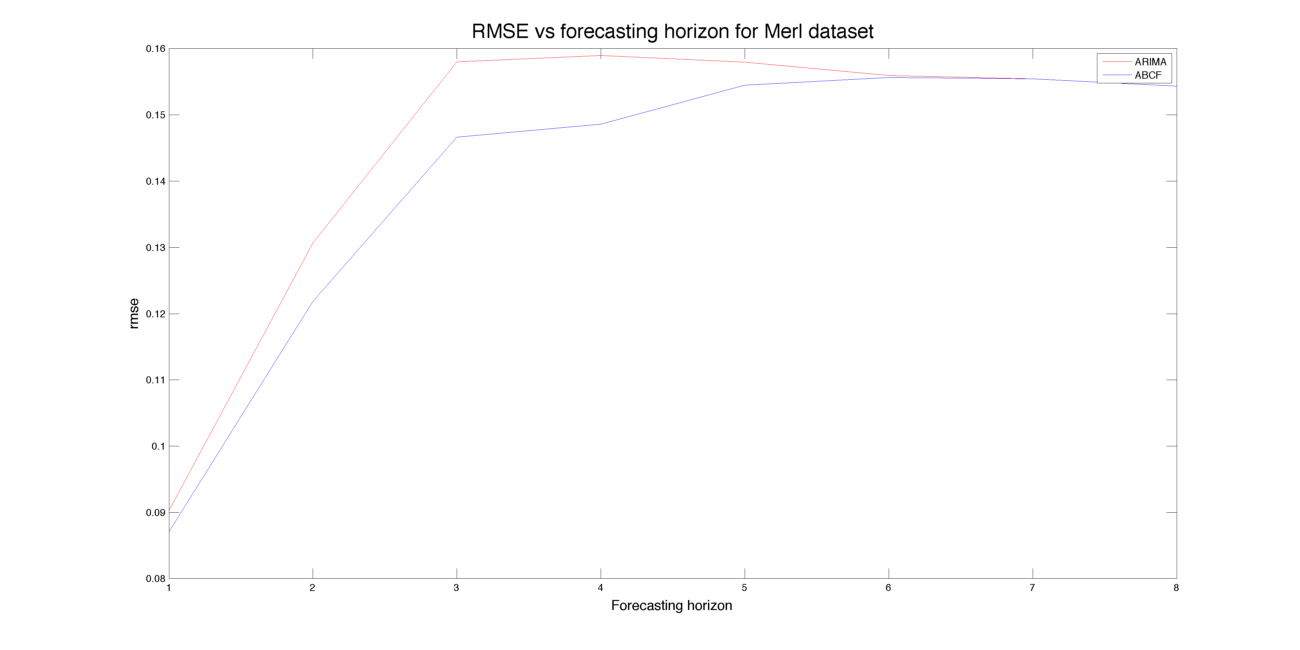
\includegraphics[width=0.37\textwidth]{rmse_merl_arima.png}
		}
		\subfigure[] {
			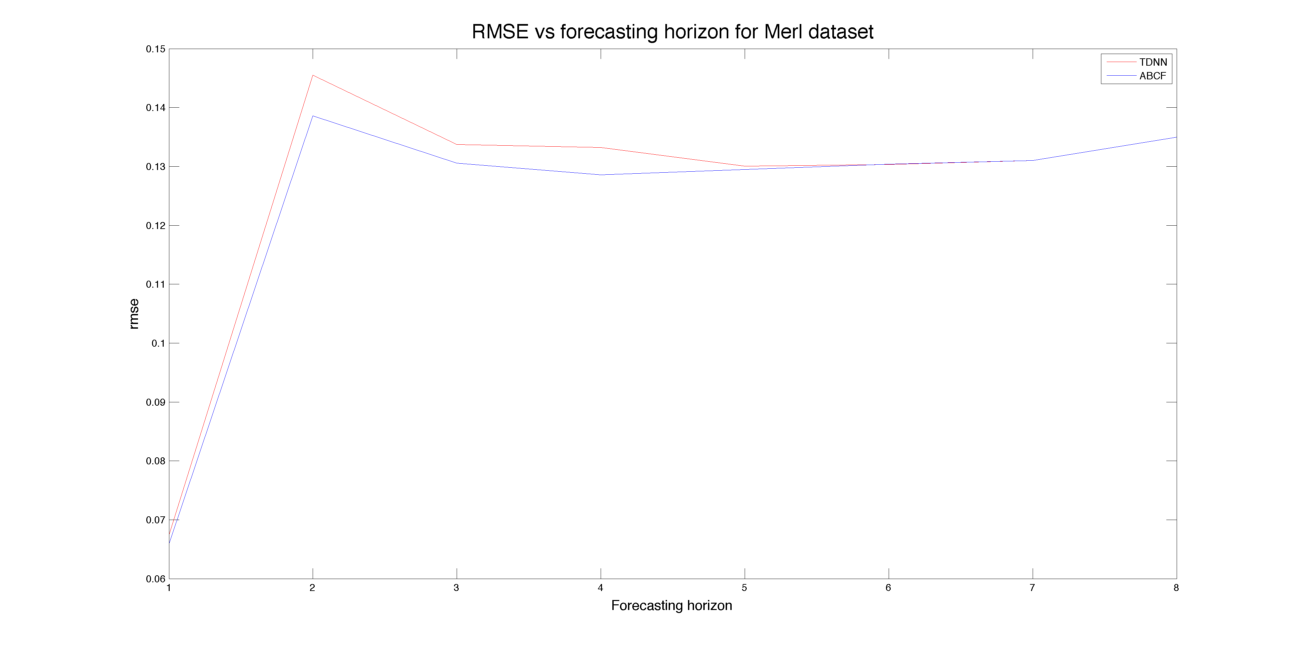
\includegraphics[width=0.37\textwidth]{rmse_merl_tdnn.png}
		}
	\end{center}
	\caption{Results for the four base forecasting algorithms for the MERL dataset and the improvements to RMSE from using our ABCF algorithm}
	\label{fig:rmse_merl_results}
\end{figure}

%brown
\begin{figure}[!h]
	\begin{center}
		\subfigure[] {
			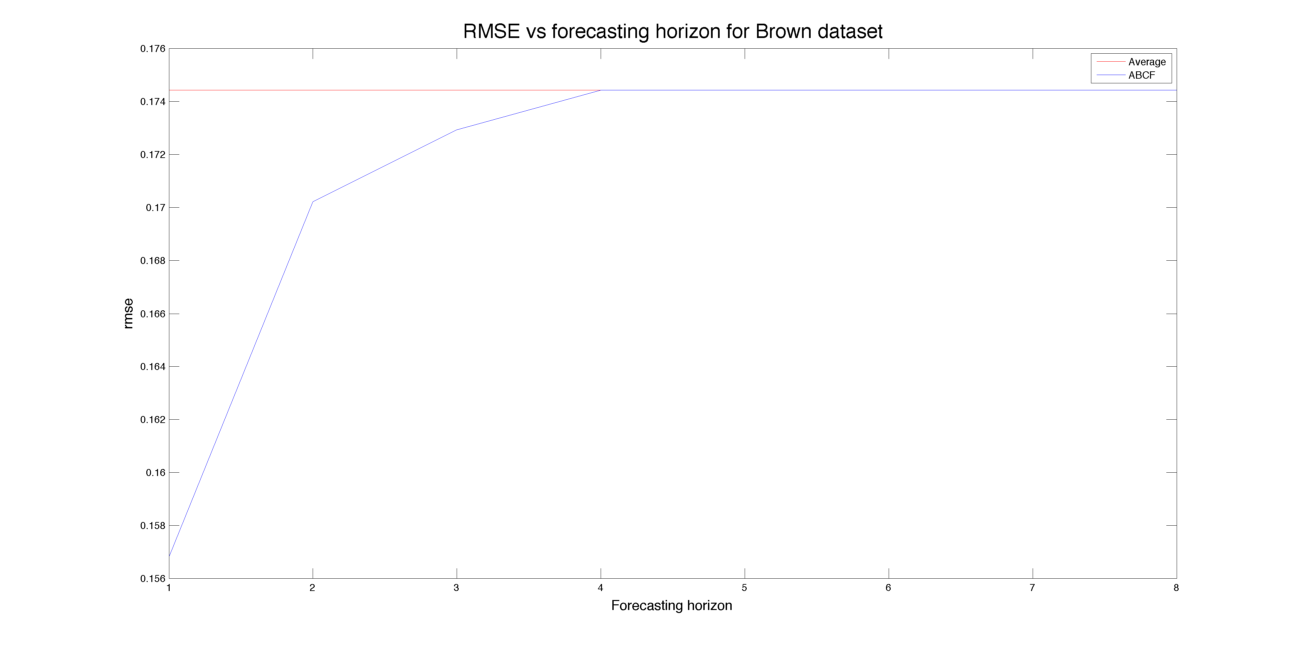
\includegraphics[width=0.37\textwidth]{rmse_brown_avg.png}
		}
		\subfigure[] {
			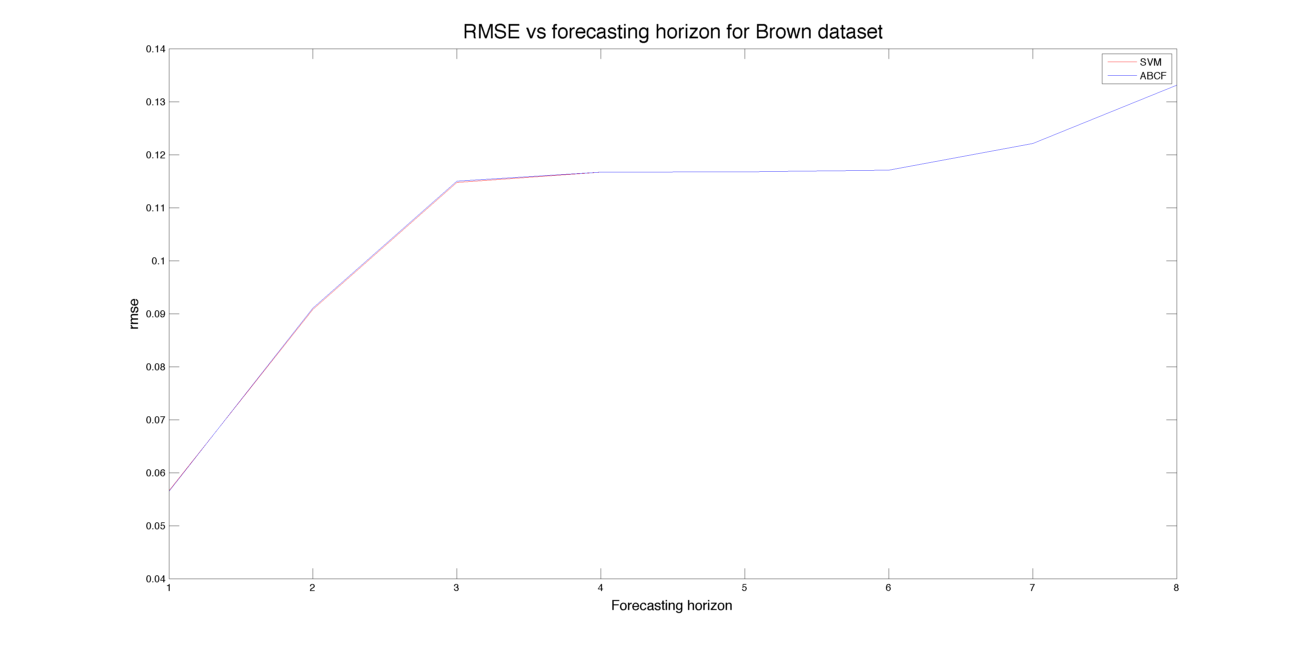
\includegraphics[width=0.37\textwidth]{rmse_brown_svm.png}
		} \\
		\subfigure[] {
			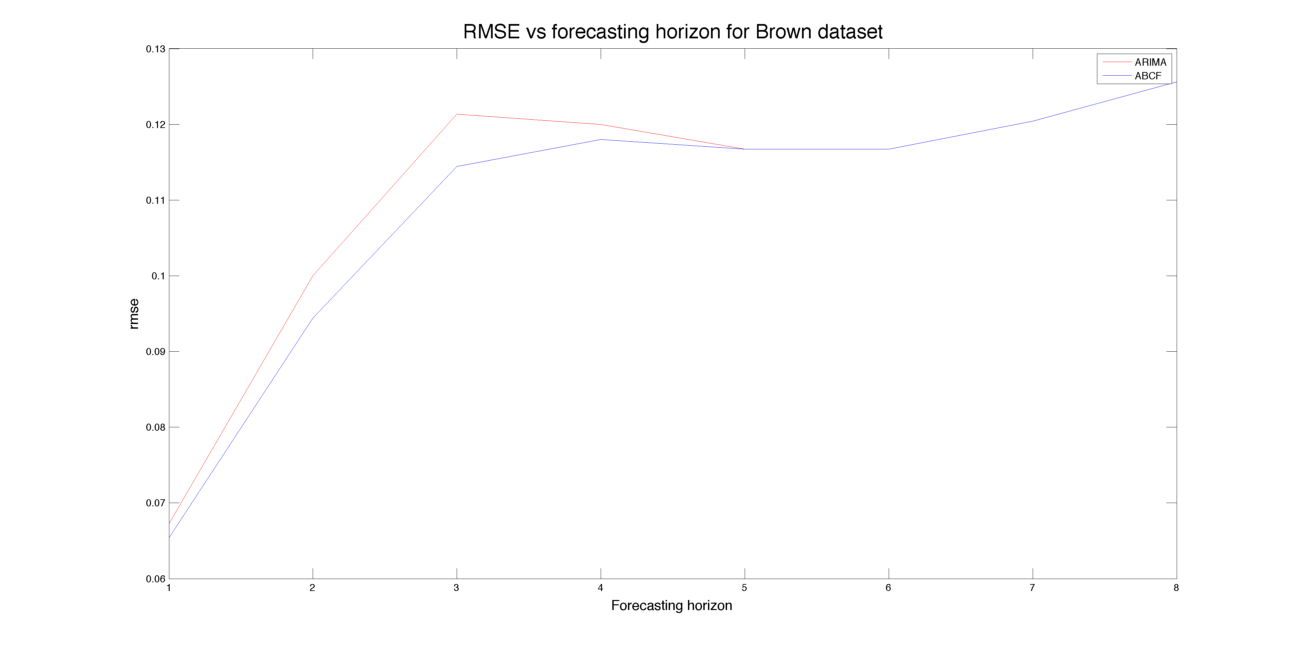
\includegraphics[width=0.37\textwidth]{rmse_brown_arima.png}
		}
		\subfigure[] {
			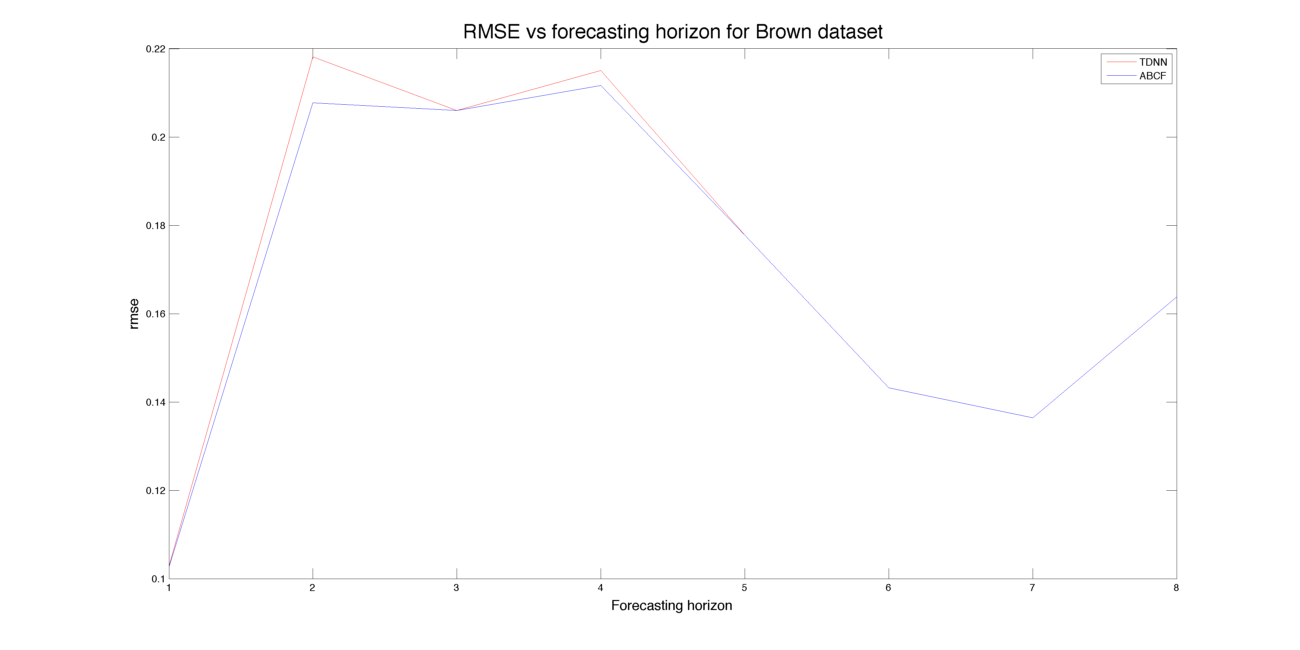
\includegraphics[width=0.37\textwidth]{rmse_brown_tdnn.png}
		}
	\end{center}
	\caption{Results for the four base forecasting algorithms for the Brown Hall dataset and the improvements to RMSE from using our ABCF algorithm}
	\label{fig:rmse_brown_results}
\end{figure}

%denver
\begin{figure}[!h]
	\begin{center}
		\subfigure[] {
			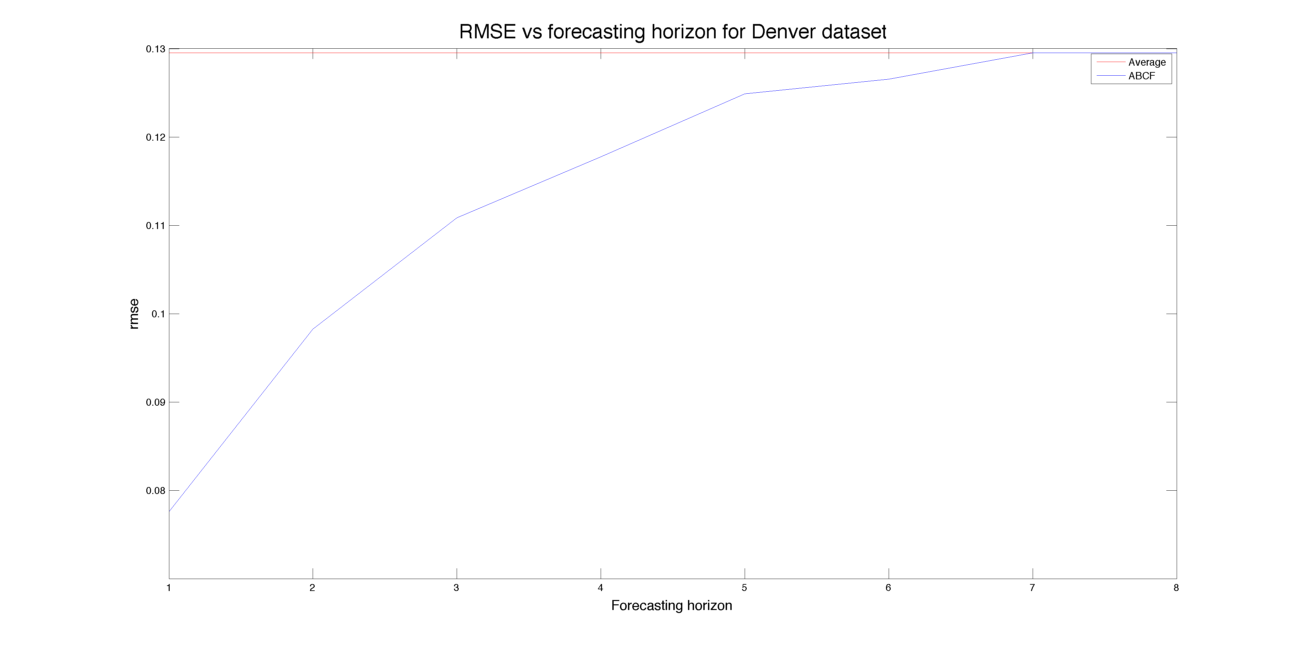
\includegraphics[width=0.37\textwidth]{rmse_denver_avg.png}
		}
		\subfigure[] {
			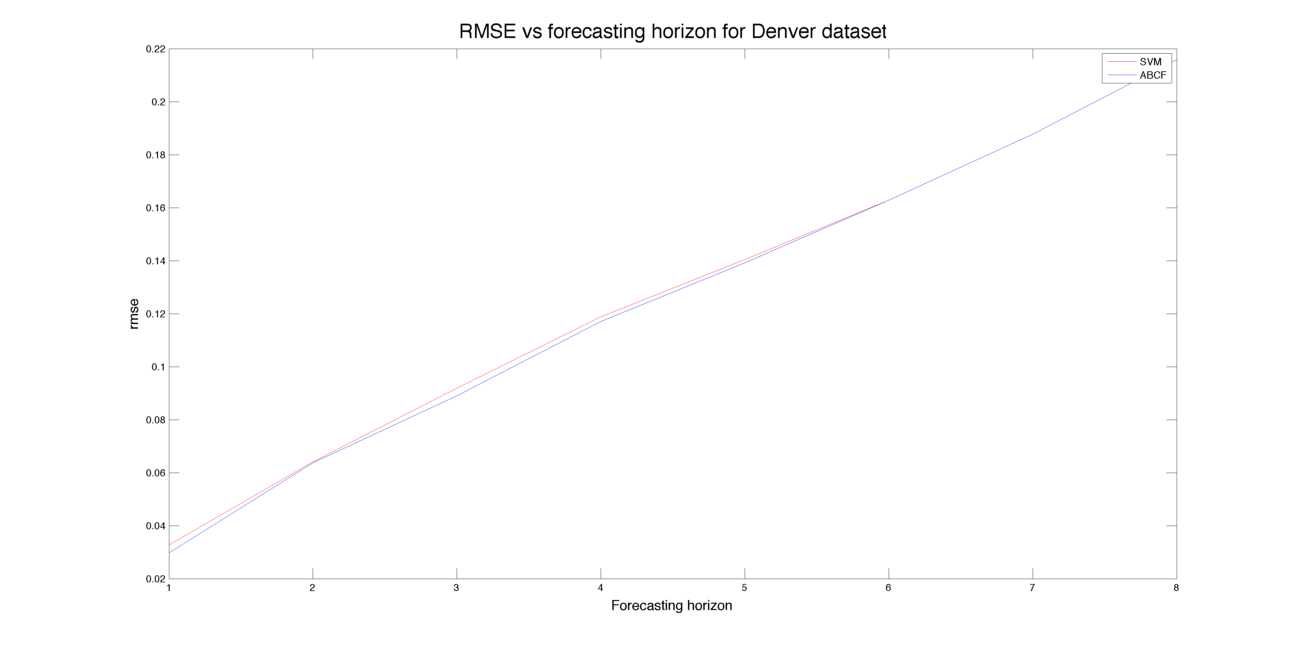
\includegraphics[width=0.37\textwidth]{rmse_denver_svm.png}
		} \\
		\subfigure[] {
			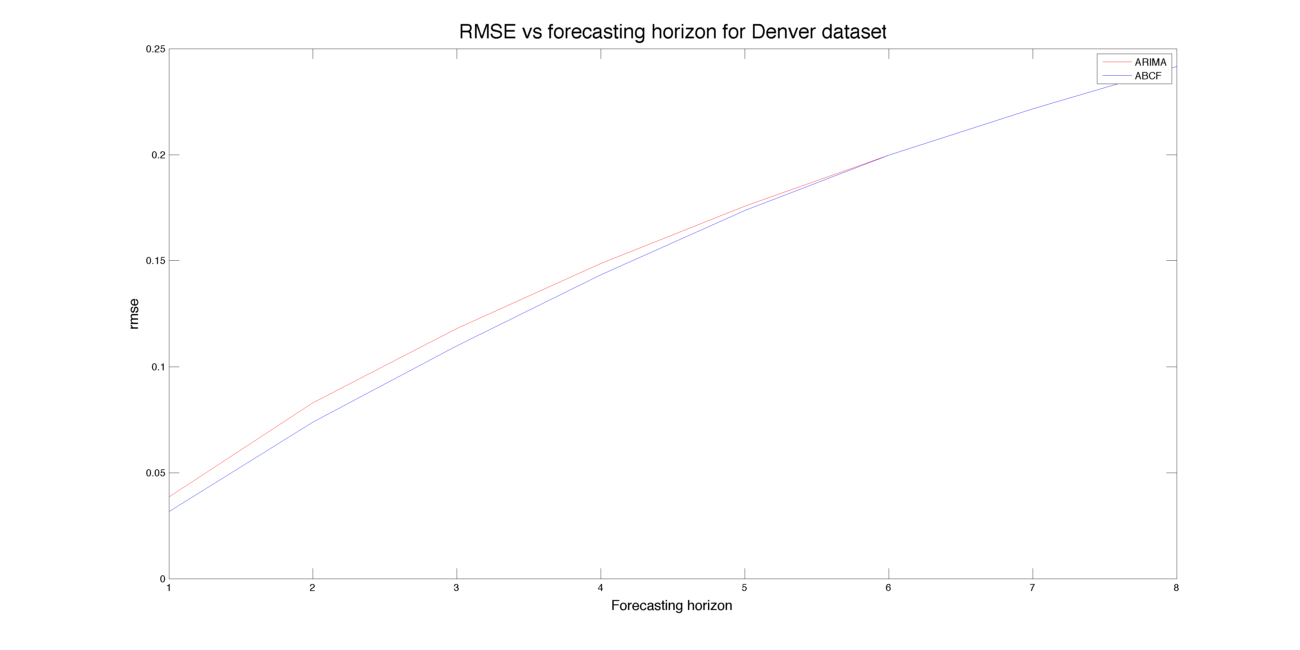
\includegraphics[width=0.37\textwidth]{rmse_denver_arima.png}
		}
		\subfigure[] {
			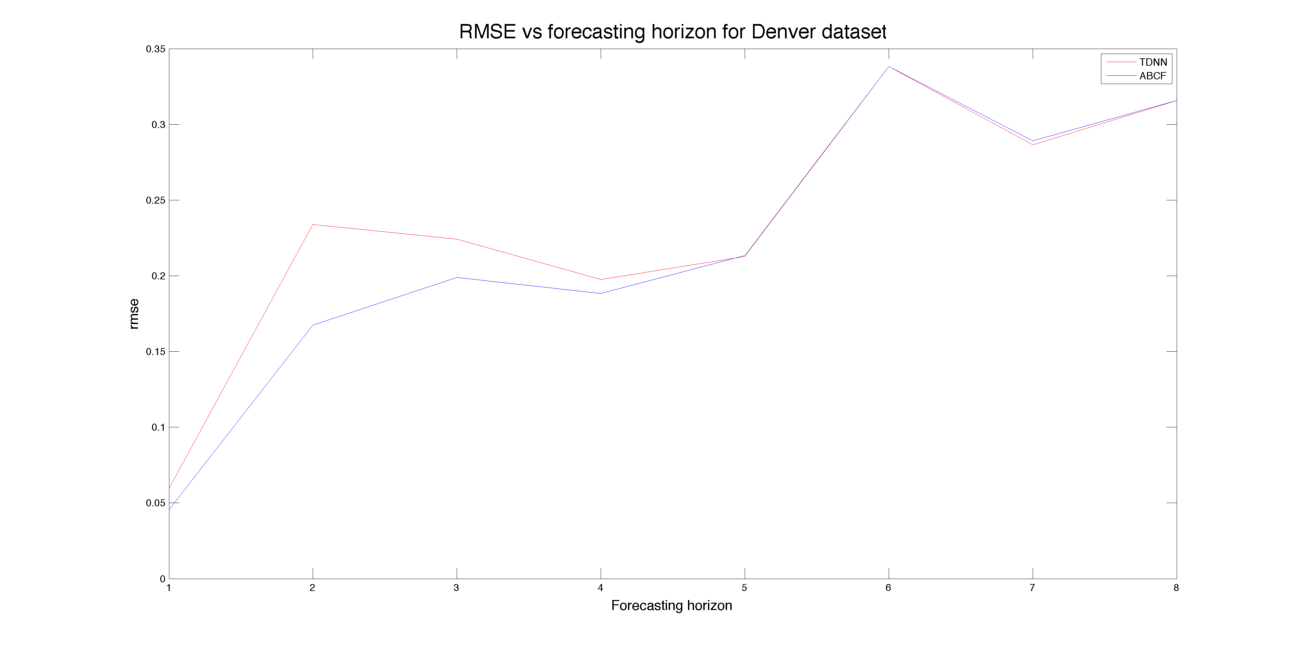
\includegraphics[width=0.37\textwidth]{rmse_denver_tdnn.png}
		}
	\end{center}
	\caption{Results for the four base forecasting algorithms for the Denver dataset and the improvements to RMSE from using our ABCF algorithm}
	\label{fig:rmse_denver_results}
\end{figure}

\newpage

%%%%%%%%%%%%%%%%%%%%%%%%%%%%%%%%%%%%%%%%%%%%%%%%%
%RMSE Results per forecaster
%%%%%%%%%%%%%%%%%%%%%%%%%%%%%%%%%%%%%%%%%%%%%%%%%
\bigskip 
\noindent \textbf{MASE Results per forecaster} \\


\begin{figure}
	\begin{center}
		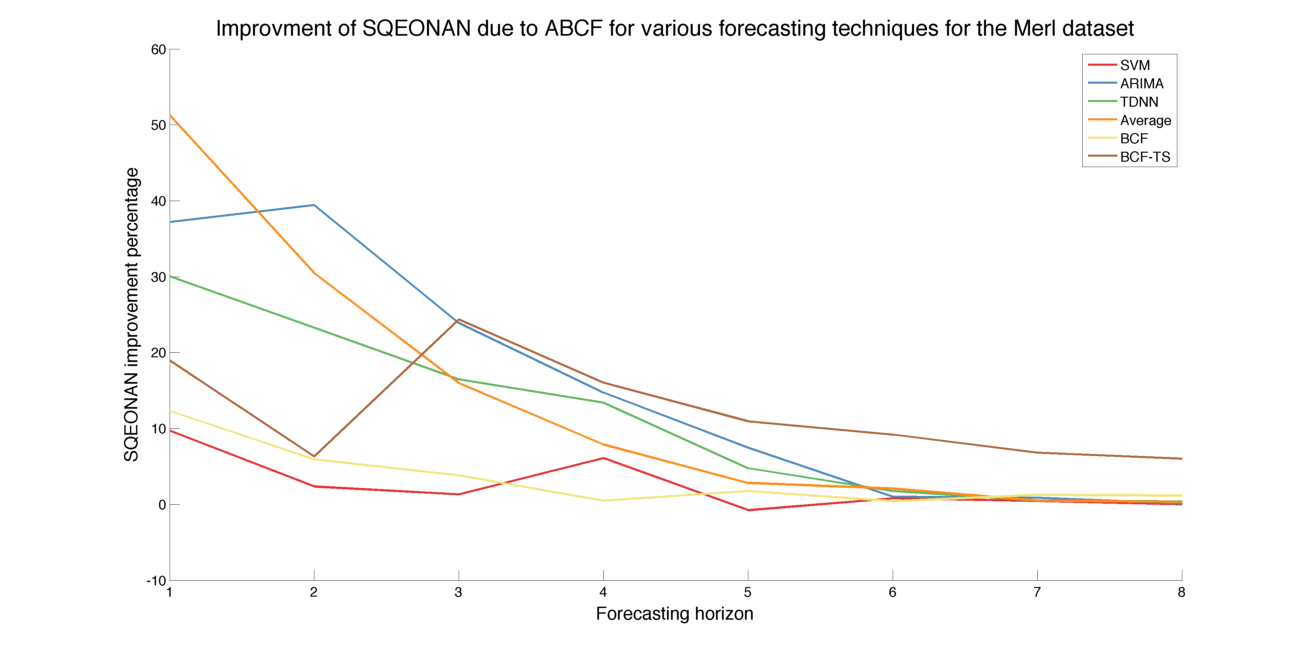
\includegraphics[width = 1.0\textwidth]{sqeonan_improvement_for_each_forecaster_for_Merl.png}
	\end{center}
	\caption{Percent improvement of applying ABCF to each forecaster for each forecasting horizon for the MERL Hall dataset}
	\label{fig:merl_sqeonan_improvement}
\end{figure}

\begin{figure}
	\begin{center}
		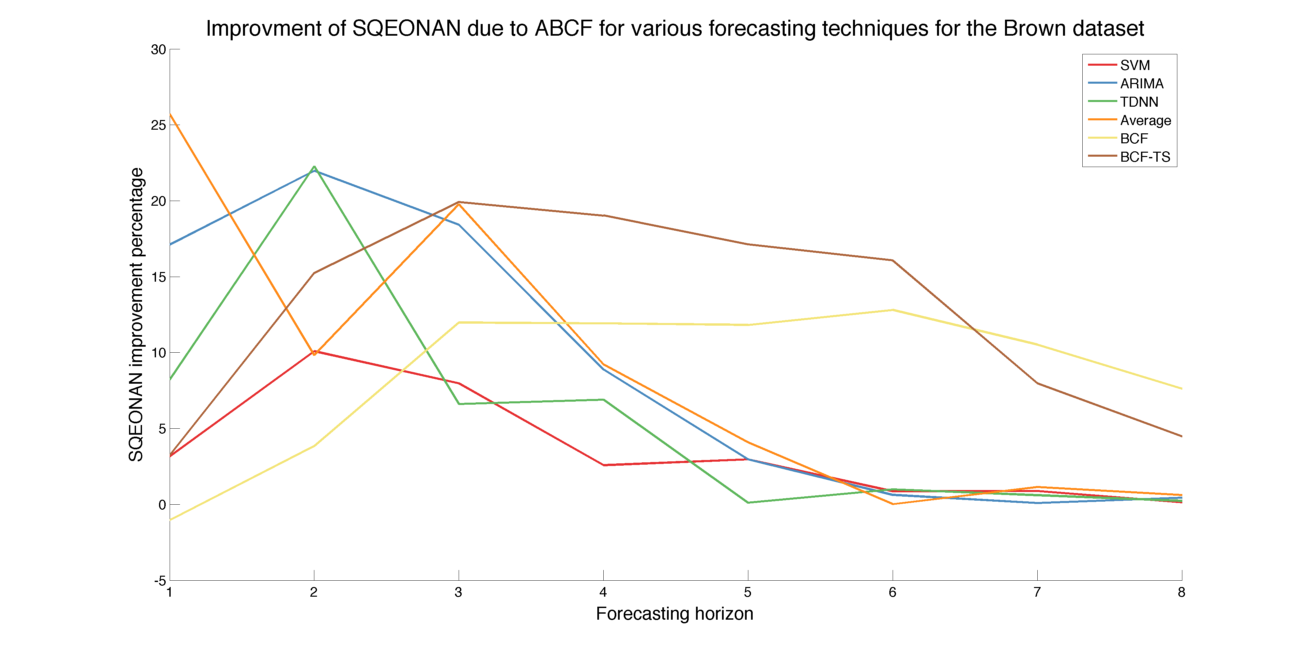
\includegraphics[width = 1.0\textwidth]{sqeonan_improvement_for_each_forecaster_for_Brown.png}
	\end{center}
	\caption{Percent improvement of applying ABCF to each forecaster for each forecasting horizon for the Brown Hall dataset}
	\label{fig:brown_sqeonan_improvement}
\end{figure}

\begin{figure}
	\begin{center}
		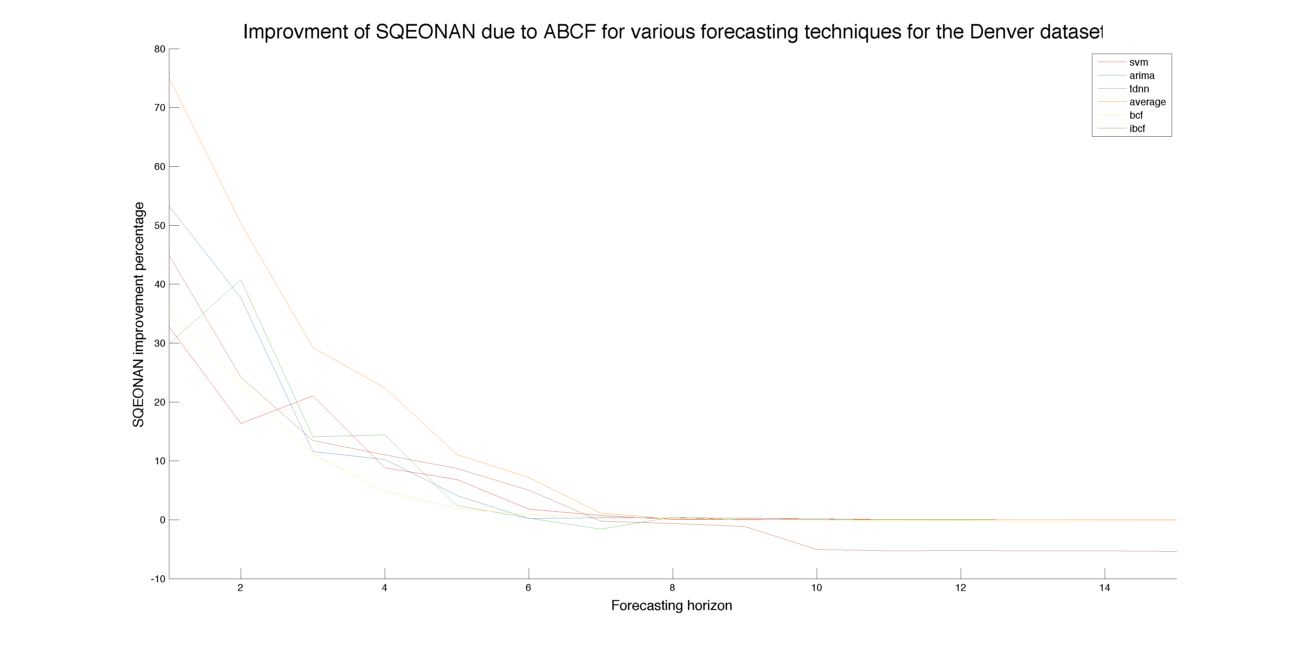
\includegraphics[width = 1.0\textwidth]{sqeonan_improvement_for_each_forecaster_for_Denver.png}
	\end{center}
	\caption{Percent improvement of applying ABCF to each forecaster for each forecasting horizon for the Denver dataset}
	\label{fig:denver_sqeonan_improvement}
\end{figure}

%TODO Include MASE Results also


\begin{figure}
	\begin{center}
		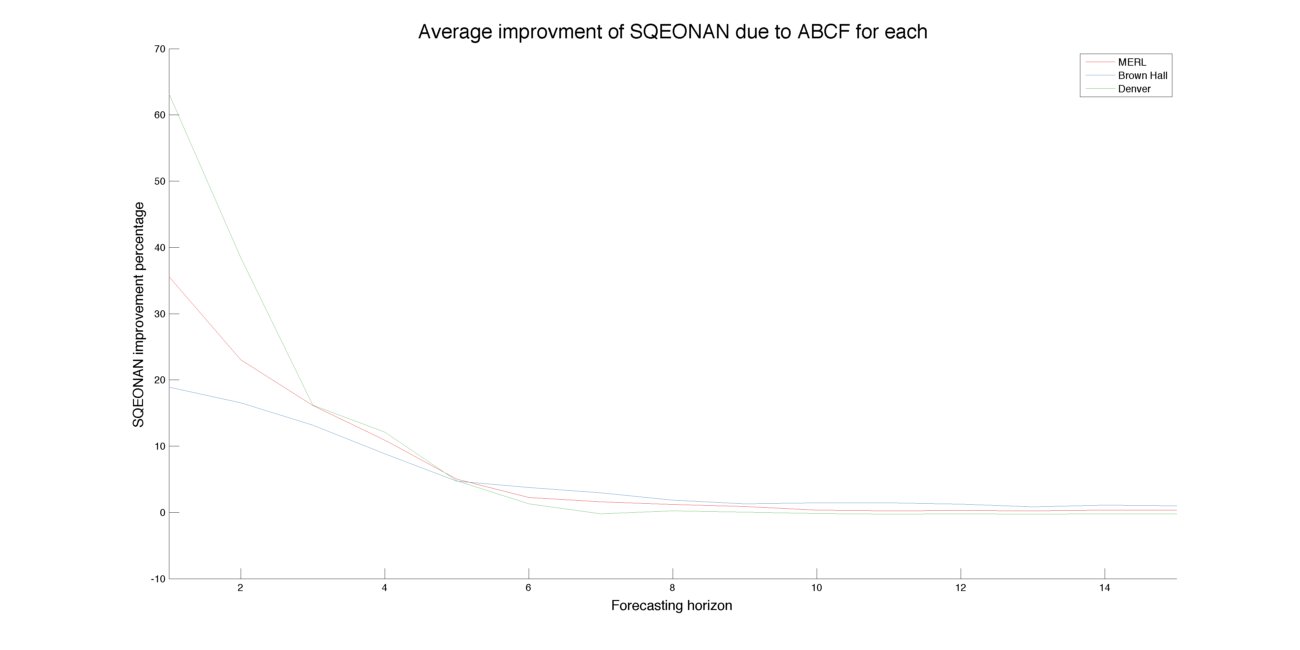
\includegraphics[width = 1.0\textwidth]{sqeonan_improvement_for_each_dataset.png}
	\end{center}
	\caption{Average percent improvement of applying ABCF to each forecaster to a given dataset.}
	\label{fig:sqeonan_improvement_all_dataset}
\end{figure}



%Reference appendix
\appendix{Figure references}\label{app:references}
This thesis was far too long in coming and far to full of various figures that do not have nice references.  
	\footnote{This footnote is simply to reference all of the unreferenced images.  Enjoy.
		\ref{fig:merl_sqeonan_improvement},
		\ref{fig:brown_sqeonan_improvement},
		\ref{fig:denver_sqeonan_improvement},
		\ref{fig:sqeonan_improvement_all_dataset},
		\ref{fig:sqe_merl_results},
		\ref{fig:sqe_brown_results},
		\ref{fig:sqe_denver_results},
		\ref{fig:rmse_merl_results},
		\ref{fig:rmse_brown_results},
		\ref{fig:rmse_denver_results}
	}